\documentclass[Modultest/CoinDispenser/CoinDispenserModulTest.tex]{subfiles}
\begin{document}
\section{CoinDispenser Hardware Modultest}

\subsection{Test af CoinSlide}
I denne seksjonen vil modul testen for CoinDetector hardwaren bli beskrevet. Hardwareen som blir testet er sklien som sorterer myntene basert på sin størrelse.\\

\\

\textbf{Krav som skal bli testet:}
\begin{enumerate}
    \item Systemet skal kun tage imod en danskfemkrone som betaling. Diameter på 28.5 mm+/- 0.5mm og tykkelse på 2.00 +/- 0.1 mm.
    \item Systemet skal returnere mønter med endiameter på 27.0 mm og under og tykkelse på2.35 mm og under
    \item Systemet skal ikke tage imod returneremønter med en diameter på 29.0 mm og overog tykkelse på over 2.35 mm
    \item Det skal detekteres mindst 98 ud af 100 gange atder indsættes en 5 krone i bolddispenser
    \item Det skal detekteres højst 2 ud af 100 gange at derindsættes en 5 krone i bolddispenser når derindsættes enhver anden dansk mønt
\end{enumerate}

\begin{figure}
    \centering
    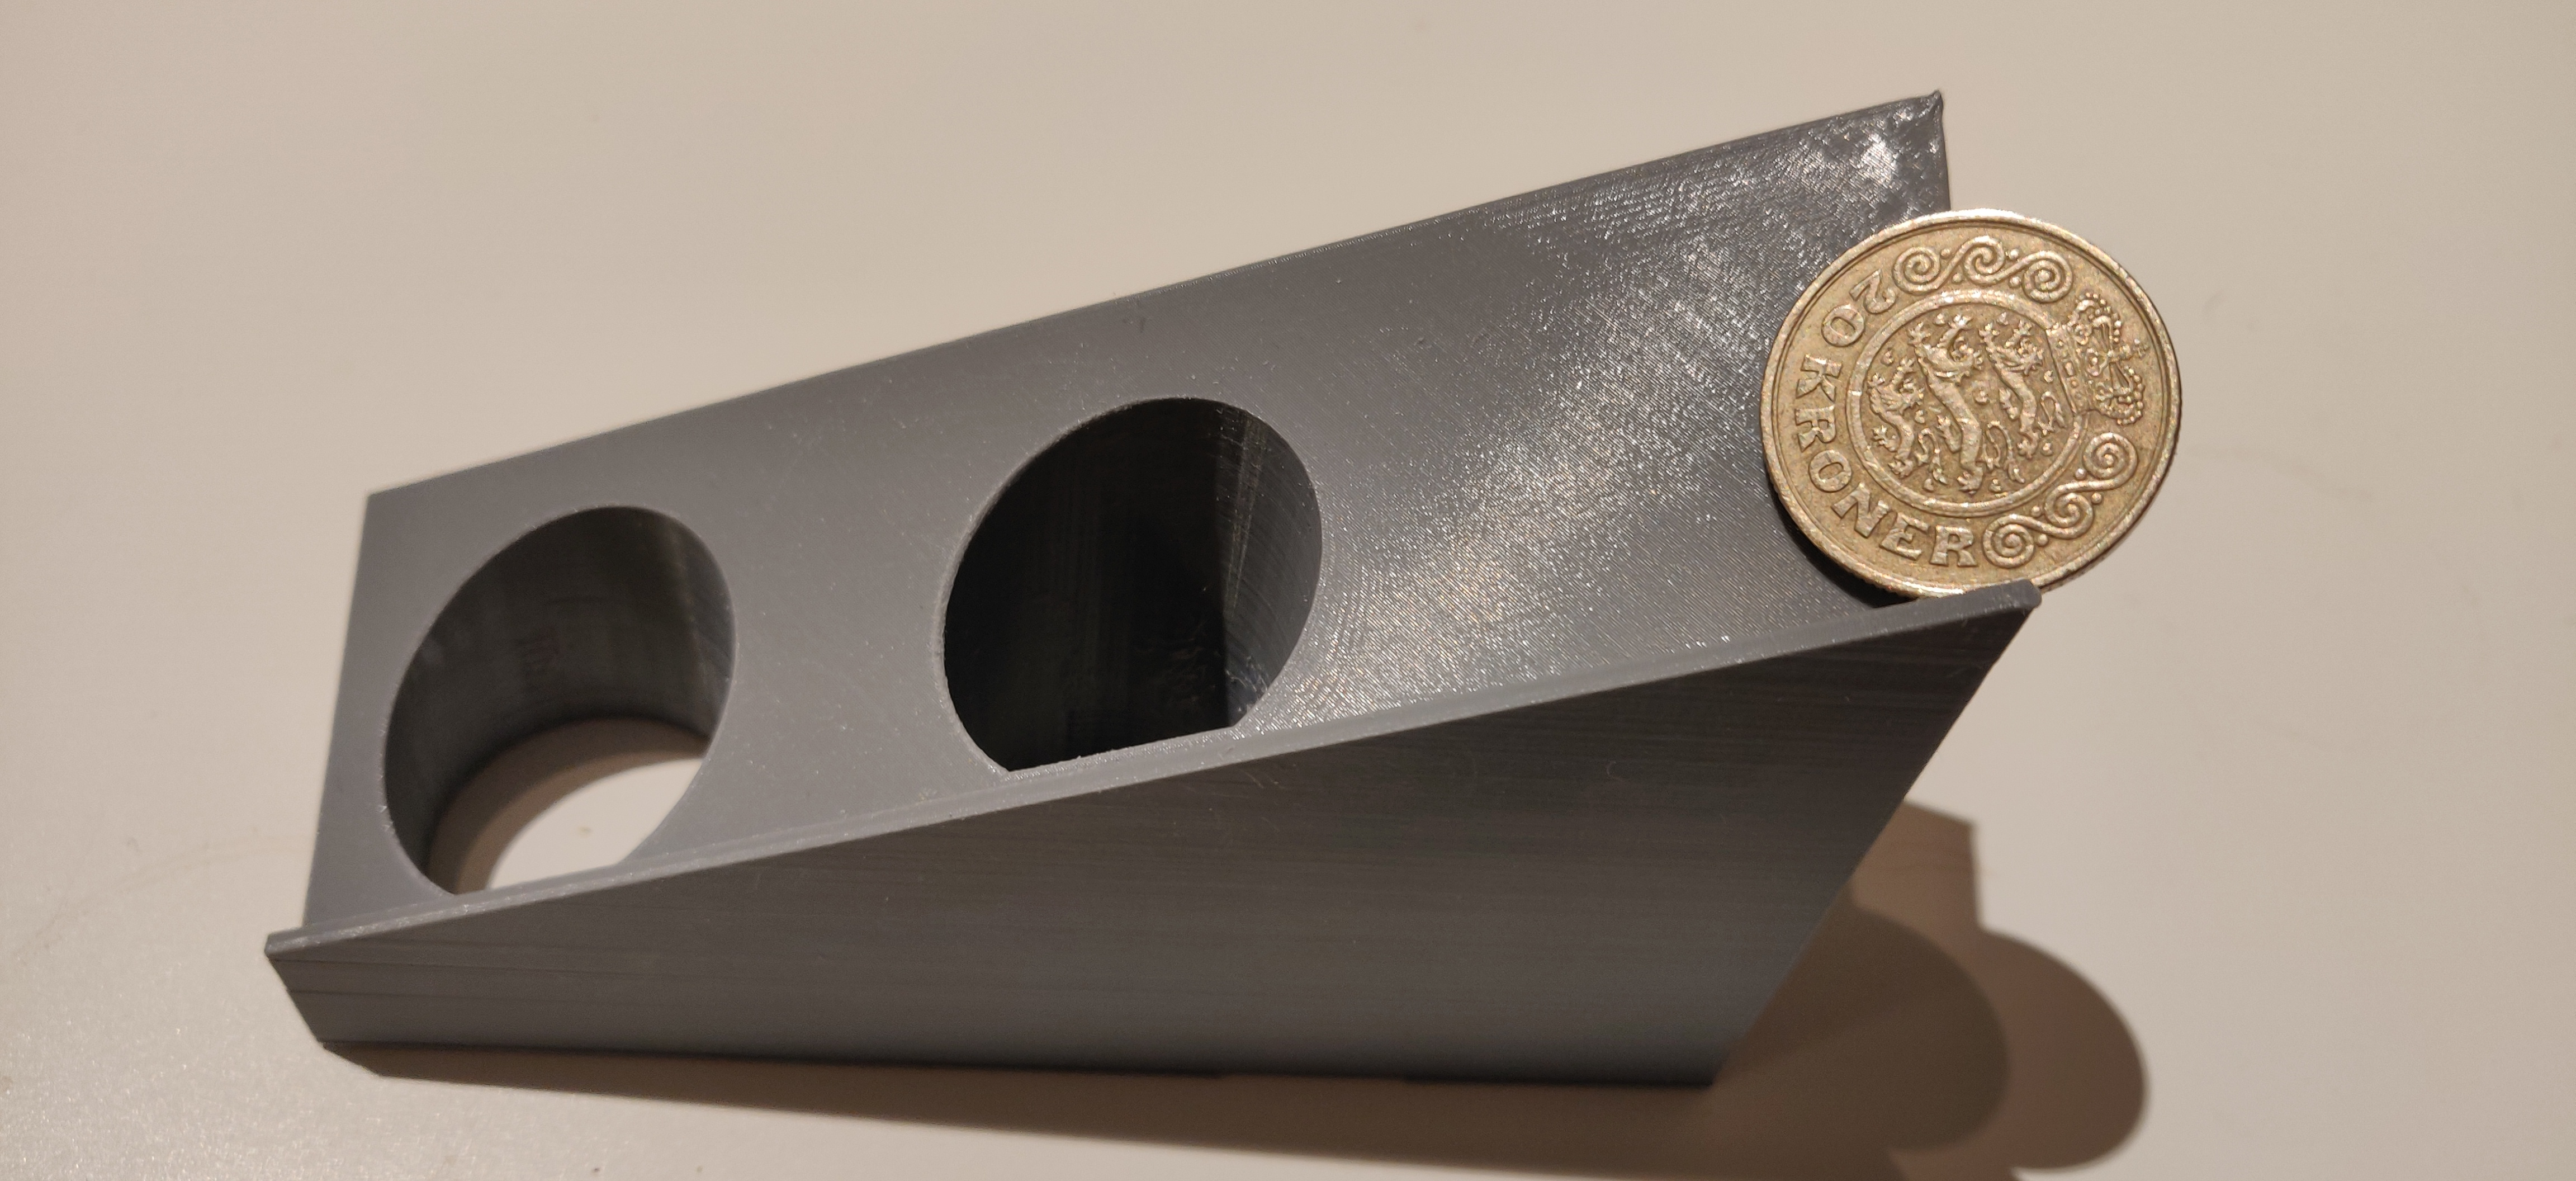
\includegraphics[width=\textwidth]{Modultest/CoinDispenser/CoinHardwareModulTest/Graphic/CoinHardwareTestSetup.jpg}
    \caption{CoinDispenser Test Setup}
    \label{fig:CoinTestSetup}
\end{figure}

Testen be utført ved sette opp sklien, legge myntene flat på toppen av skien og la dem skli ned. Dette ble gjennomført 200 ganger både for 5 kroner og 20 kr. Under er resultatene presentert:

\subsection{Resultater Test 1}
\begin{table}[H]
\Large
\centering
\begin{tabular}{|l|l|l|}
\hline

\textbf{Mynt} & \textbf{Forsøk} & \textbf{Feil} \\ \hline
5 kr          & 200             & 9             \\ \hline
20 kr         & 200             & 1             \\ \hline

\end{tabular}
\end{table}

\subsection{Refleksion Test 1}

Som vi kan se ble 5 kr myntene feil sortert 4,5\% av gangene som ikke er innenfor det akseptable feilmarginet. Derfor ble det gjennomført noen endringer på sklien og deretter ble 300 nye målinger ble tatt.

\subsection{Resultater Test 2}
\begin{table}[H]
\Large
\centering
\begin{tabular}{|l|l|l|}
\hline
\textbf{Mynt} & \textbf{Forsøk} & \textbf{Feil} \\ \hline
5 kr          & 300             & 1             \\ \hline
20 kr         & 300             & 2             \\ \hline
\end{tabular}
\end{table}
\subsection{Refleksion Test 2}
Som man kan se er målingene nå innenfor feilmarginet og testen anses som bestått.

\end{document}